\documentclass[aspectratio=169]{beamer}
\usetheme{metropolis}
\title{Automate the boring stuff with \texttt{pytorch-lightning}}
\date{13 May, 2020}
\author{Jacob Nilsson}
\institute{Luleå University of Technology}

% Packages
\usepackage[]{minted} 
\usepackage[]{graphicx} 
\usepackage[]{verbatim} 
\usepackage[]{hyperref} 

% Macros
\newcommand{\alertsymb}{
\includegraphics[height=0.7cm]{alert.png}} 
\newcommand{\livecode}{\Large \centering \alertsymb \hspace{1em}
	LIVE CODING EXAMPLE \hspace{1em} \alertsymb}

% Colors
\definecolor{LTUblue}{cmyk}{1,0.5,0,0.6}
\definecolor{LTUorange}{cmyk}{0,0.46,0.93,0}
\setbeamercolor{palette primary}{bg=LTUblue,fg=white}
\setbeamercolor{alerted text}{fg=LTUorange}

% Minted options
\setminted[python]{
	tabsize=4, 
	python3=true}

\begin{document}
	\maketitle
	\section{What's the boring stuff?}
	\begin{frame}{An example of boilerplate code}
		\livecode
	\end{frame}

	\begin{frame}{An example of boilerplate code}
		\begin{minipage}[b]{0.45\textwidth}
			With boring stuff:\\[1em]

			\inputminted[firstline=4, lastline=7]{python}{
			../boilerplate-example-finished.py}
		\end{minipage}\hfill
		\begin{minipage}[b]{0.45\textwidth}
			Without boring stuff:\\[1em]

			\inputminted[firstline=11, lastline=14]{python}{
			../boilerplate-example-finished.py}
		\end{minipage}
	\end{frame}

	\begin{frame}{Flexibility vs. Readability}
		\begin{minipage}[b]{0.45\textwidth}
			Higher flexibility\\
			Messier code\\
			More error prone:\\[1em]

			\inputminted[firstline=4, lastline=7]{python}{
			../boilerplate-example-finished.py}
		\end{minipage}\hfill
		\begin{minipage}[b]{0.45\textwidth}
			Lower flexibility\\
			Cleaner code\\
			Less error prone:\\[1em]

			\inputminted[firstline=11, lastline=14]{python}{
			../boilerplate-example-finished.py}
		\end{minipage}
	\end{frame}

	\begin{frame}{Opinions on PyTorch vs TensorFlow}
		\vfill
		\begin{minipage}[t]{0.45\textwidth}
			\textbf{PyTorch}:\\\small

			Flexible models (``normal'' code)*\\
			Easy debugging (\texttt{print()} works)*\\

			\alert<2>{Deployment is manual} and requires a lot of boilerplate code
		\end{minipage}\hfill
		\begin{minipage}[t]{0.45\textwidth}
			\textbf{TensorFlow}:\\\small

			Models are difficult to change*\\
			Difficult debugging*\\

			\alert<2>{Deployment is streamlined}
		\end{minipage}\\[5em]
		\centering \tiny *Common thoughts about PyTorch vs. TensorFlow online
	\end{frame}

	\section{Introduction to \texttt{pytorch-lightning}}

	\begin{frame}{What is \texttt{pytorch-lightning}}
		Pytorch-lightning is a tool to organize pytorch code.\\
		Pytorch-lightning organizes code into 3 categories:
		\begin{enumerate}
			\item Research code
			\item Engineering code (Boilerplate)
			\item Non-essential research code (logging)
		\end{enumerate}
	\end{frame}

	\begin{frame}{Comparing pure torch to \texttt{pytorch-lightning}}
		\livecode
	\end{frame}

	\begin{frame}{Research code}
		\centering
		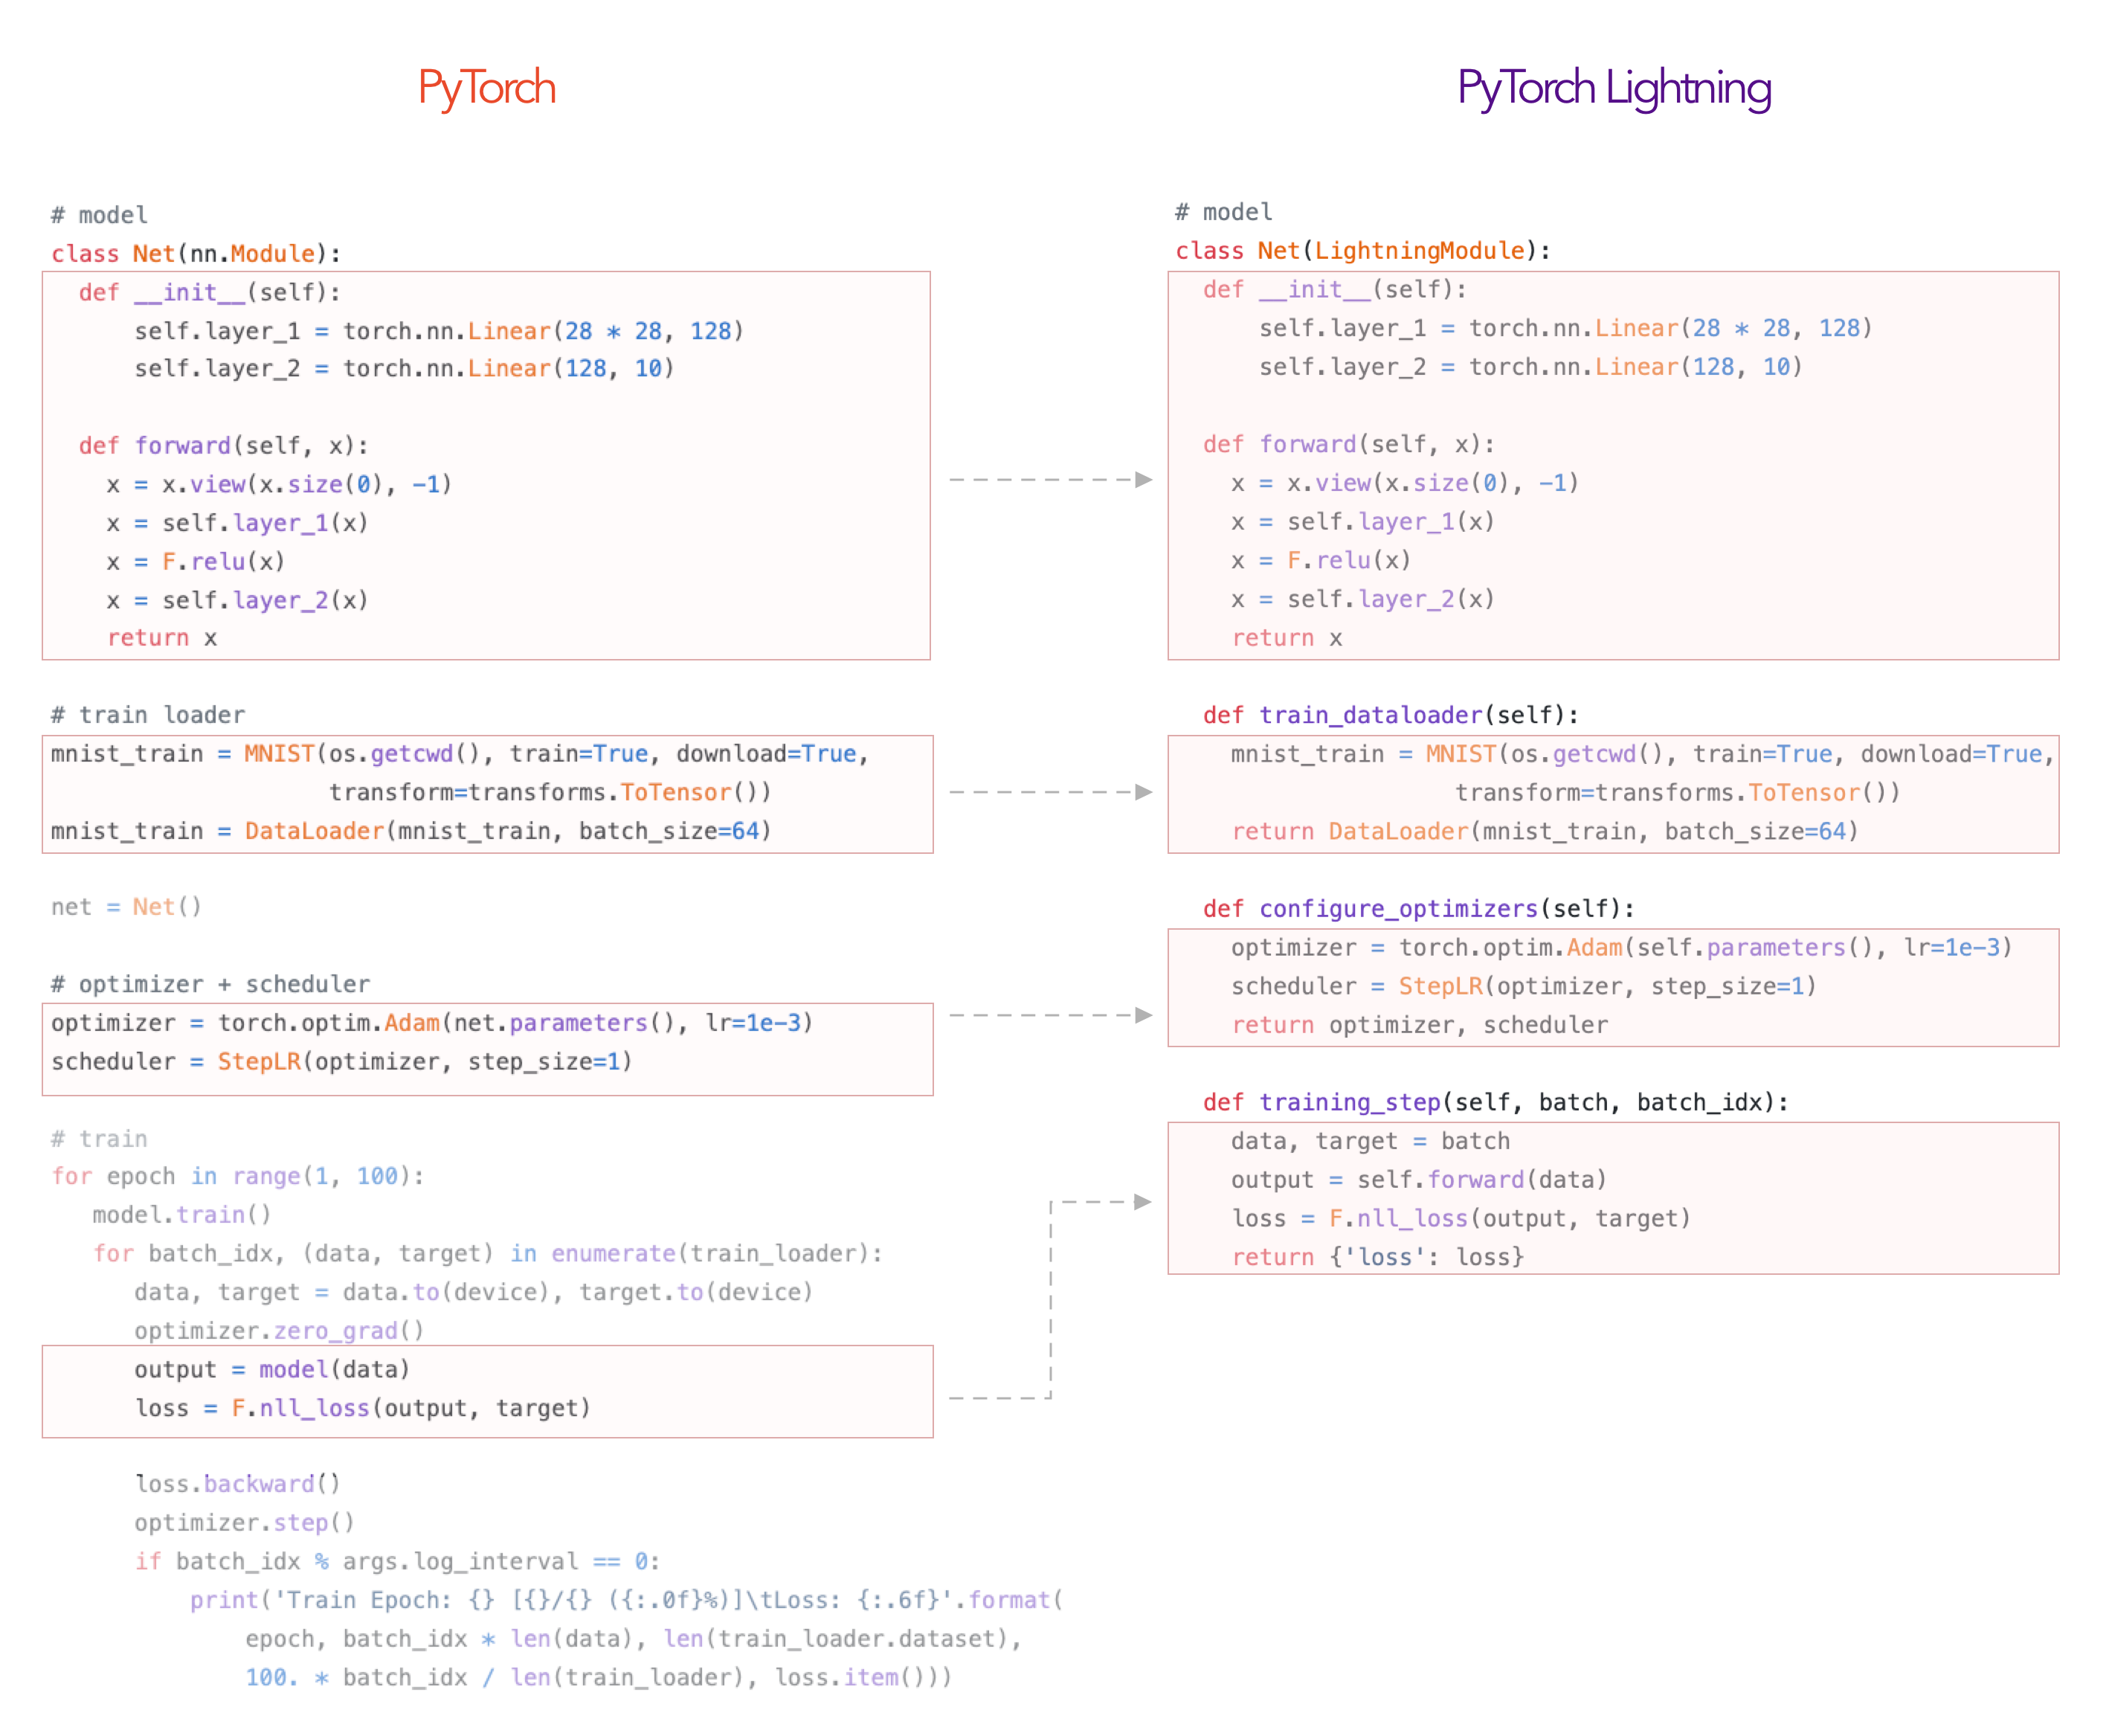
\includegraphics[height=0.9\textheight]{pt_to_pl.png}
	\end{frame}

	\begin{frame}{Engineering code}
		\centering
		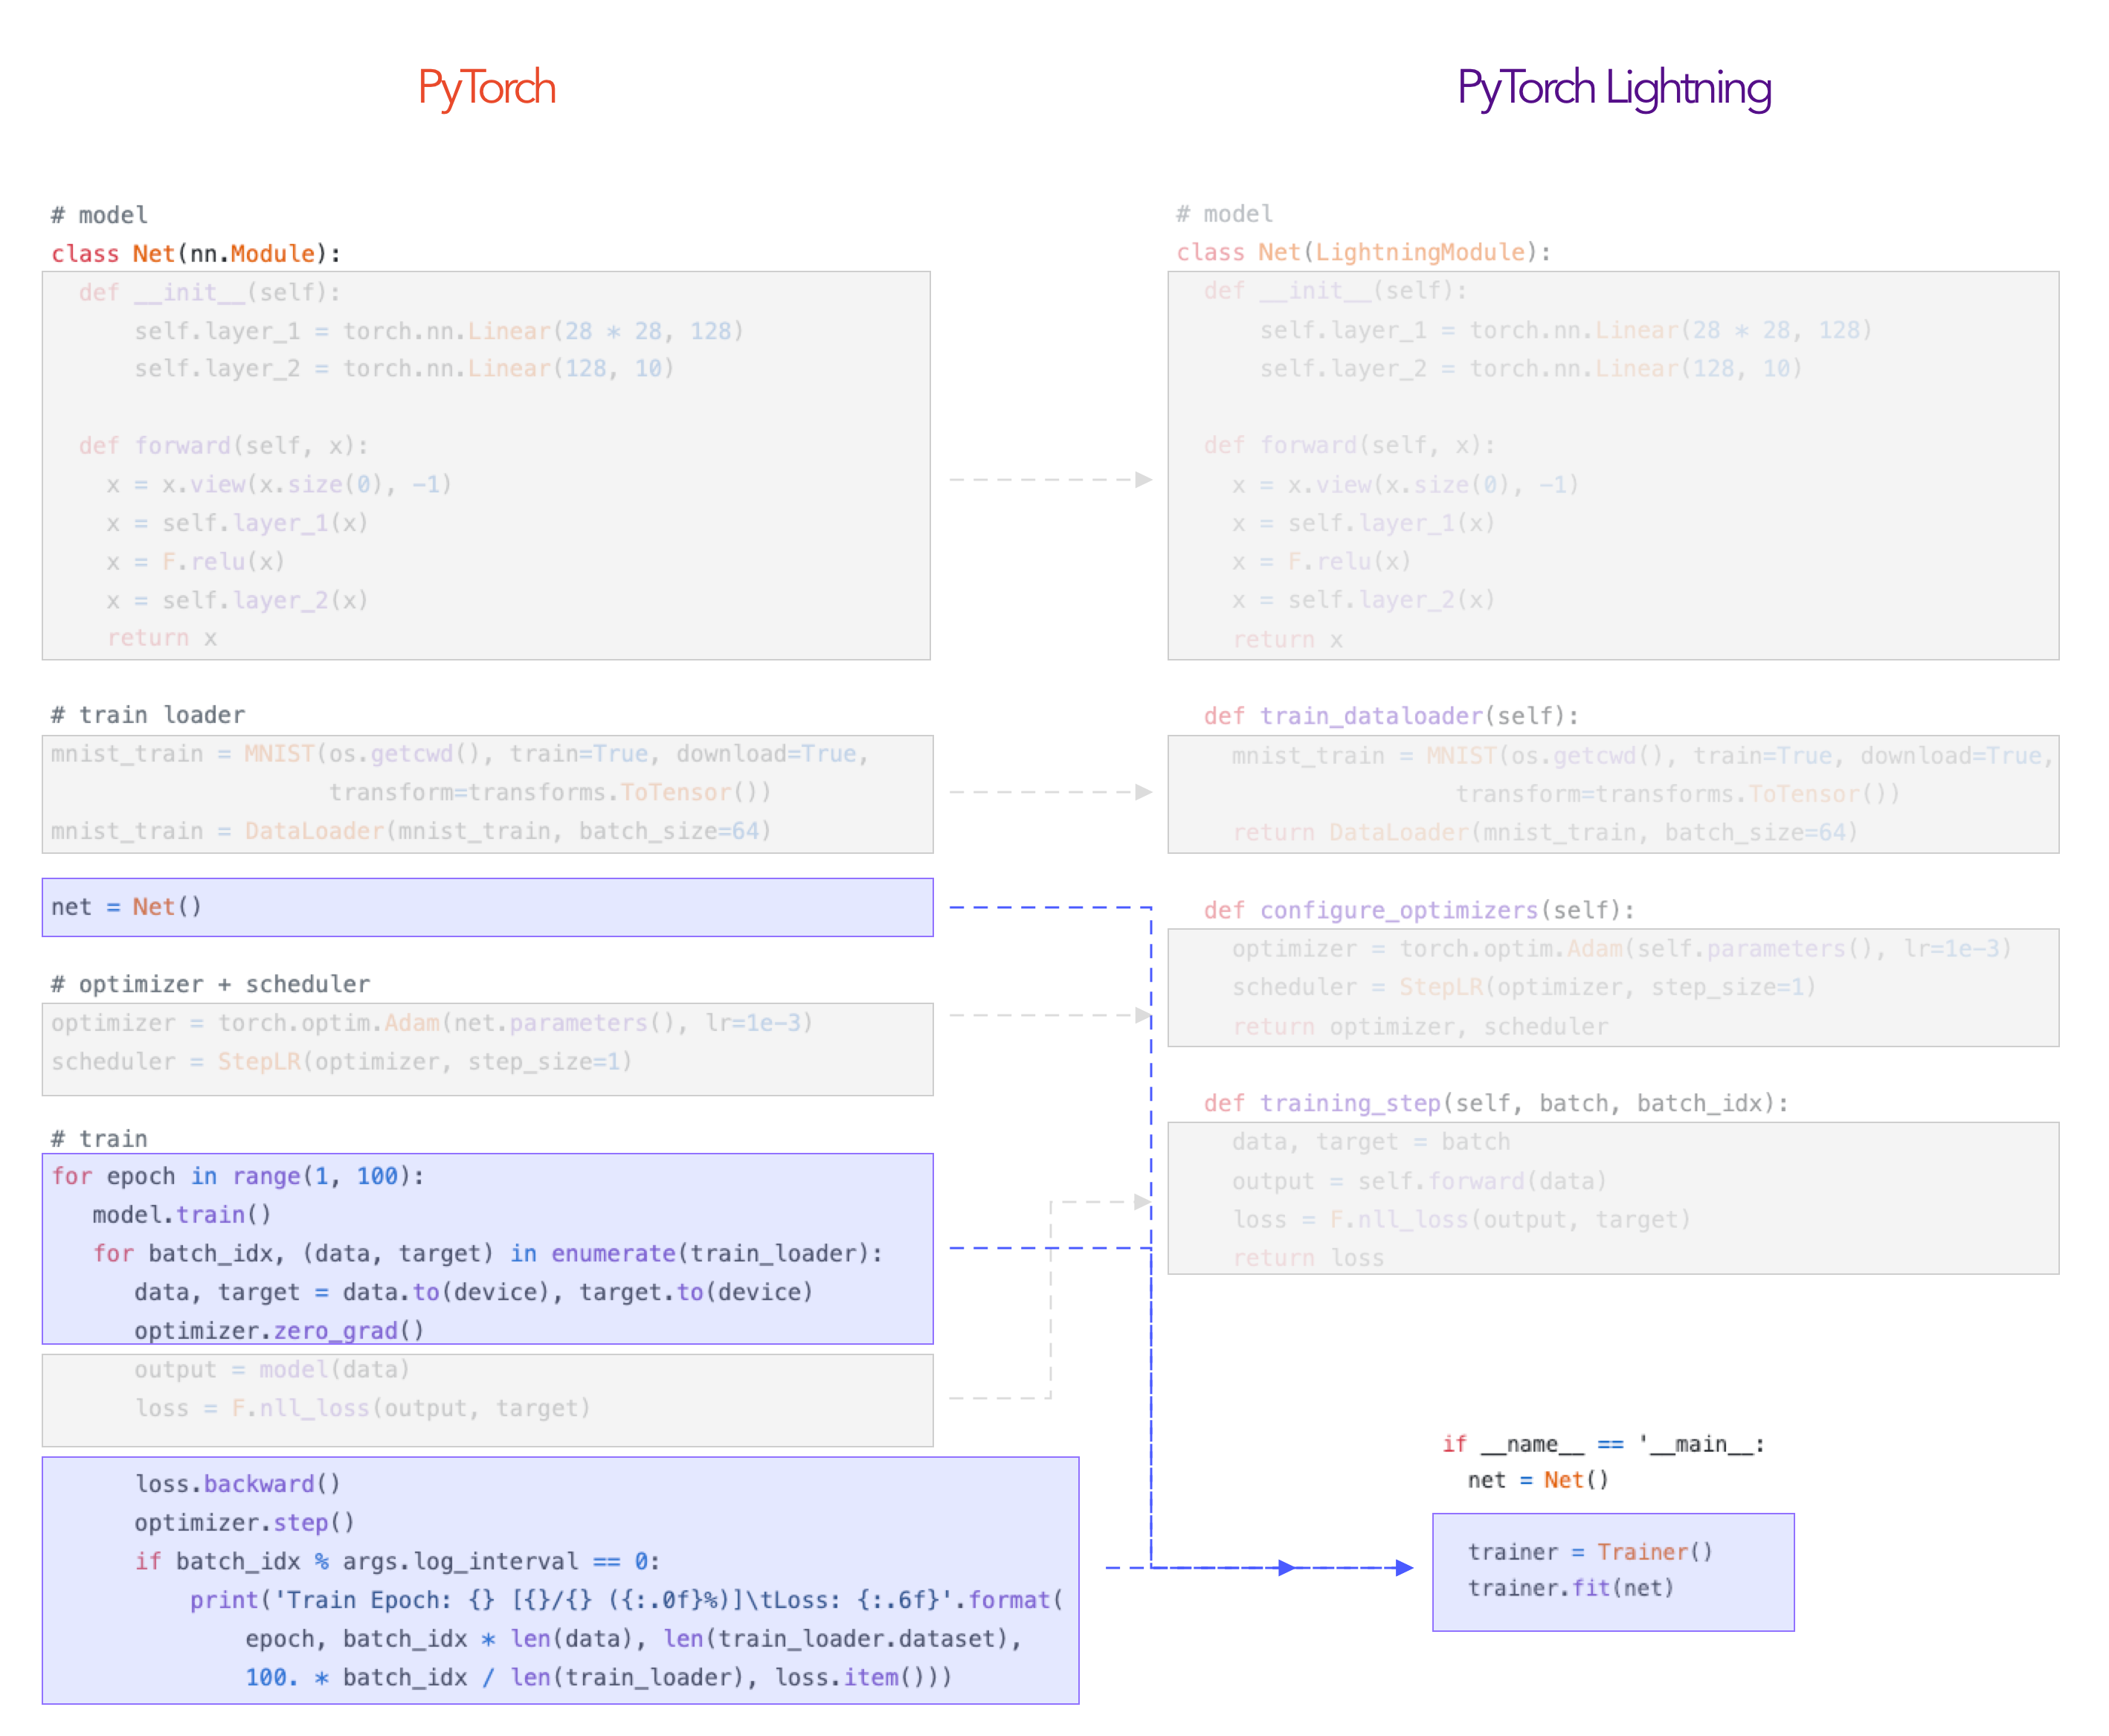
\includegraphics[height=0.9\textheight]{pt_trainer.png}
	\end{frame}

	\begin{frame}{Summary thus far}
		\centering
		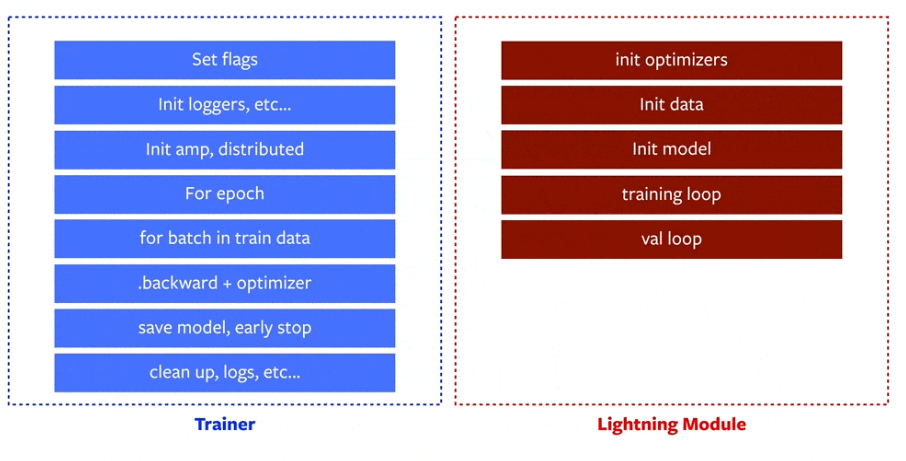
\includegraphics[height=0.7\textheight]{research_engineering.png}
	\end{frame}

	\begin{frame}[standout]
		\LARGE Question break
	\end{frame}

	\section{Validation, Testing, Progress Bar, and Logging}

	\begin{frame}[fragile]{Validation}
		To do validation, you add two methods and a dataloader:
		\begin{minted}[autogobble]{python}
			def validation_step(self, batch, batch_idx):
				""" Calculate validation for batch """

			def validation_epoch_end(self, outputs):
				""" Average results over all batches """

			def val_dataloader(self):
				""" Returns a validation dataloader """
		\end{minted}
		\vfill
		For testing, replace \texttt{validation} with \texttt{test}
	\end{frame}

	\begin{frame}[fragile]{Progress Bar and Logging}
		All \texttt{\_step} and \texttt{\_epoch\_end} methods \emph{must} return a dictionary where you can choose what is logged and shown in the progress bar.
		\begin{minted}[autogobble, fontsize=\footnotesize]{python}
			def training_step(self, batch, batch_idx):
				""" 
				
				"""
				return {'loss': loss} # Mandatory for training_step

			def validation_epoch_end(self, batch, batch_idx):
				""" 
				
				"""
				return {'progress_bar': pb_dict, # dict of progress bar
					'log': {'val_loss', val_loss} # dict of variables to log
		\end{minted}
	\end{frame}

	\begin{frame}[fragile]{Customizable loggers}
		Logging is done automatically done with Tensorboard by default, but can be swapped to any other logger compatible with Pytorch Lightning, see \url{https://pytorch-lightning.readthedocs.io/en/latest/loggers.html}. For example TestTube:

		\begin{minted}[autogobble, fontsize=\footnotesize]{python}
			def main():
				from pytorch_lightning.loggers import TestTubeLogger
				ttlogger = TestTubeLogger('tb_logs', name='my_model')
				trainer = pl.Trainer(logger=ttlogger)
		\end{minted}
	\end{frame}

	\begin{frame}{Full code example}
		\livecode
	\end{frame}

	\begin{frame}{Summary of section}
		To add \emph{validation} or \emph{testing} functionality, you add \texttt{step} and \texttt{epoch\_end} (collation) methods, as well as a dataloader for each functionality.
		\vfill
		Logging is easily added, and logger behaviour can be changed.
	\end{frame}
	
	\section{Debugging}
	
	\begin{frame}[fragile]{Validation sanity checks}
		Pytorch Lightning runs a few validation steps (5 by default) before training to find errors before costly training begins. Can be customized:
		\begin{minted}[autogobble, fontsize=\footnotesize]{python}
			trainer = Trainer(num_sanity_val_steps=5)
		\end{minted}
	\end{frame}

	\begin{frame}[fragile]{Fast dev run}
		To quickly check that the model runs through all steps correctly, you can set the \texttt{fast\_dev\_run} flag:

		\begin{minted}[autogobble, fontsize=\footnotesize]{python}
			trainer = Trainer(fast_dev_run=True)
		\end{minted}
	\end{frame}

	\begin{frame}[fragile]{Overfitting checks}
		You can tell the trainer to overfit on a small subset of your data to check that the loss goes to 0.
		\begin{minted}[autogobble, fontsize=\footnotesize]{python}
			trainer = pl.Trainer(
				overfit_pct=0.01, # Overfits on 1% of the data
				training_percent_check=0.01, # Overfits on 1% of the training data
		\end{minted}
	\end{frame}

	\section{Customizing the training loop}

	\begin{frame}[fragile]{Callbacks}
		Non-essential functionality is put in callbacks, some important ones are already defined such as early stopping and model checkpointing
		\begin{minted}[autogobble, fontsize=\footnotesize]{python}
			from pytorch_lightning.callbacks import EarlyStopping, \
													ModelCheckpoint

			early_stopping = EarlyStopping('val_loss')
			checkpoint_callback = ModelCheckpoint(filepath='my/path/')

			trainer = Trainer(early_stop_callback=early_stopping,
							  checkpoint_callback=checkpoint_callback)
		\end{minted}
		
	\end{frame}

	\begin{frame}{Callbacks}
		Each callback can be further customized to suit specific tasks, and new callbacks can be written if needed, see \small\url{https://pytorch-lightning.readthedocs.io/en/latest/callbacks.html}.
	\end{frame}

	\begin{frame}[fragile]{Model Hooks}
		The \emph{model hooks} are the methods that comprise the model interface. \texttt{training\_step} is a model hook.

		Each hook represent a behaviour of the model, and all hooks can be changed to change the behaviour.
	\end{frame}

	\begin{frame}[fragile]{Hooks example: \texttt{on\_epoch\_start}}
		Used if you have something you need to do at the start of each epoch:

		\begin{minted}[autogobble, fontsize=\footnotesize]{python}
			class Net(pl.LightningModule):
				def on_epoch_start():
					print('new epoch started')
					self.a *= 1.1
		\end{minted}
	\end{frame}

	\begin{frame}{More Hooks}
		Consult the documentation for more hooks, some are very specific and they are open to suggestions for new hooks. 
		
		\url{https://pytorch-lightning.readthedocs.io/en/latest/api/pytorch_lightning.core.hooks.html}
		
	\end{frame}

	\section{Summary}

	\begin{frame}{Summary}
		Pytorch Lightning is a framework for Pytorch that strives to reduce the amount of engineering code in your projects, letting you focus on research.

		Logging is automatic.

		Debugging functionality is built-in.

		Little flexibility is lost due to flexible callbacks and model hooks.

		``Standardizes'' training code in Pytorch (to those who use it).
	\end{frame}

	\begin{frame}[standout]
		Questions
	\end{frame}

\end{document}

